%% Template for MLP Coursework 3

%% Based on  LaTeX template for ICML 2017 - example_paper.tex at 
%%  https://2017.icml.cc/Conferences/2017/StyleAuthorInstructions

\documentclass{article}
\usepackage[T1]{fontenc}
\usepackage{amssymb,amsmath}
\usepackage{txfonts}
\usepackage{microtype}
\usepackage{xspace}
\xspaceaddexceptions{\%}

% Lists with less spacoing between items
\usepackage{paralist}

% For figures
\usepackage{graphicx}
\usepackage{subfig} 

% For citations
\usepackage{natbib}

% For algorithms
\usepackage{algorithm}
\usepackage{algorithmic}

% the hyperref package is used to produce hyperlinks in the
% resulting PDF.  If this breaks your system, please commend out the
% following usepackage line and replace \usepackage{mlp2017} with
% \usepackage[nohyperref]{mlp2017} below.
\usepackage[hyphens]{url}
\urlstyle{same}
\usepackage{hyperref}

% Packages hyperref and algorithmic misbehave sometimes.  We can fix
% this with the following command.
\newcommand{\theHalgorithm}{\arabic{algorithm}}


% Set up MLP coursework style (based on ICML style)
\usepackage{mlp2022}
\mlptitlerunning{MLP Coursework 3 -- Interim Report (\groupNumber)}
\bibliographystyle{icml2017}


\DeclareMathOperator{\softmax}{softmax}
\DeclareMathOperator{\sigmoid}{sigmoid}
\DeclareMathOperator{\sgn}{sgn}
\DeclareMathOperator{\relu}{relu}
\DeclareMathOperator{\lrelu}{lrelu}
\DeclareMathOperator{\elu}{elu}
\DeclareMathOperator{\selu}{selu}
\DeclareMathOperator{\maxout}{maxout}







%% You probably do not need to change anything above this comment

%% REPLACE this with your project title, group ID and list of student numbers for the group
\def\projectTitle{Title}
\def\groupNumber{G000}
\def\studentNumbers{sXXXXXXX, sYYYYYYY, sZZZZZZZ}

\begin{document} 

\twocolumn[
\mlptitle{\projectTitle: Interim Report}

\centerline{\groupNumber\ (\studentNumbers)}

\vskip 7mm
]

\begin{abstract} 
The abstract should be a few sentences (100--200 words) long,  providing a concise summary of the contents of your report including the key research question(s) addressed, the methods explored, the data used, and the findings of the experiments.
\end{abstract} 

\section{Introduction}
\label{sec:intro}
This document provides a template for the MLP coursework 3 interim report.  This template structures the report into sections, which you may use,or you can structure it differently if you wish.  If you want to use subsections within a section that is fine. In this template the text in each section will include a very brief outline of what you should include in each section, along with some practical LaTeX examples (for example figures, tables, algorithms).  Your document should be no longer than \textbf{five pages},  with an additional page (or more!) allowed for references.

You should give a broad introduction to the project, including citations to related work. Your aim here is to explain why the project is addressing an interesting topic, and how it relates to things that have been done in the area.

You should make clear what are the aims and objectives of the project, what are the research questions being addressed.  Be precise. In this section you should make clear what the project's contribution is: how is it different to what is already done. 

The interim report should state the objectives of the project, which are related to the research questions. What experiments do you plan to carry out? You can differentiate between core objectives, and optional objectives you hope to achieve if things go well. The conclusions in your final report should relate to these objectives.

Use bibtex to organise your references -- in this case the references are in the file \verb+example-refs.bib+.  Here is a an example reference \citep{langley00}.  



\section{Data set and task} 
Clearly describe the data set and task you will be exploring.  If the data requires any preprocessing, then explain this.  The description should be in enough detail such that your work would be reproducible by another group.  Describe how you will evaluate the task (for example, classification accuracy).  Use citations where appropriate.

\section{Methodology}
Explain clearly the technical methodology, the models and algorithms that are used.  Approaches that were covered in the lectures can be described briefly, but if you are using modifications to such approaches make sure these are clearly described. Again use citations to the literature. Avoid pasting or paraphrasing the methodology directly from the cited work. Instead consider why you are using these approaches, and how they can best be presented in the context of your work. Keep examples consistent with your domain, and notation consistent with your paper. Consider also how you might have adapted the approaches to work in your case. 

If you present algorithms, you can use the \verb+algorithm+ and \verb+algorithmic+ environments to format pseudocode (for instance, Algorithm~\ref{alg:example}). These require the corresponding style files, \verb+algorithm.sty+ and \verb+algorithmic.sty+ which are supplied with this package. 

\begin{algorithm}[ht]
\begin{algorithmic}
   \STATE {\bfseries Input:} data $x_i$, size $m$
   \REPEAT
   \STATE Initialize $noChange = true$.
   \FOR{$i=1$ {\bfseries to} $m-1$}
   \IF{$x_i > x_{i+1}$} 
   \STATE Swap $x_i$ and $x_{i+1}$
   \STATE $noChange = false$
   \ENDIF
   \ENDFOR
   \UNTIL{$noChange$ is $true$}
\end{algorithmic}
  \caption{Bubble Sort}
  \label{alg:example}
\end{algorithm}


\section{Experiments}
\label{sec:expts}
The interim report should include some experimental results.  In most cases these will be baseline experiments. Baseline experiments refer to experiments conducted using well-understood approaches against which you can compare later results.  In particular, you need to be able to justify that the baseline performance is a reasonable hurdle for your solutions to overcome. This is in contrast to a benchmark, which would be the performance you would need to beat to indicate positive findings. Baselines are used, among other things, to test that both your benchmark(s) and proposed solutions have been properly set up and trained. For example if you were exploring a new data set, the baselines might include linear networks and deep neural networks with different numbers of hidden layers;  if you were exploring a different approach to regularisation, then the baselines would include no regularisation, and conventional techniques such as L1, L2, and dropout.  You can include the results of any further experiments in your interim report.



Present the experimental results clearly and concisely.  Usually a result is in comparison or contrast to a result from another approach please make sure that these comparisons/contrasts are clearly presented.  You can facilitate comparisons either using graphs with multiple curves or (if appropriate, e.g. for accuracies) a results table. You need to avoid having too many figures, poorly labelled graphs, and graphs which should be comparable but which use different axis scales. A good presentation will enable the reader to compare trends in the same graph -- each graph should summarise the results relating to a particular research (sub)question.

There is no need to include code or specific details about the compute environment.

As before, your experimental sections should include graphs (for instance, figure~\ref{fig:sample-graph}) and/or tables (for instance, table~\ref{tab:sample-table})\footnote{These examples were taken from the ICML template paper.}, using the \verb+figure+ and \verb+table+ environments, in which you use \verb+\includegraphics+ to include an image (pdf, png, or jpg formats).  Please export graphs as 
\href{https://en.wikipedia.org/wiki/Vector_graphics}{vector graphics}
rather than \href{https://en.wikipedia.org/wiki/Raster_graphics}{raster
files} as this will make sure all detail in the plot is visible.
Matplotlib supports saving high quality figures in a wide range of
common image formats using the
\href{http://matplotlib.org/api/pyplot_api.html\#matplotlib.pyplot.savefig}{\texttt{savefig}}
function. \textbf{You should use \texttt{savefig} rather than copying
the screen-resolution raster images outputted in the notebook.} An
example of using \texttt{savefig} to save a figure as a PDF file (which
can be included as graphics in a \LaTeX document is given in the coursework document.

If you need a figure or table to stretch across two columns use the \verb+figure*+ or \verb+table*+ environment instead of the \verb+figure+ or \verb+table+ environment.  Use the \verb+subfigure+ environment if you want to include multiple graphics in a single figure.

\begin{figure}[tb]
\vskip 5mm
\begin{center}
\centerline{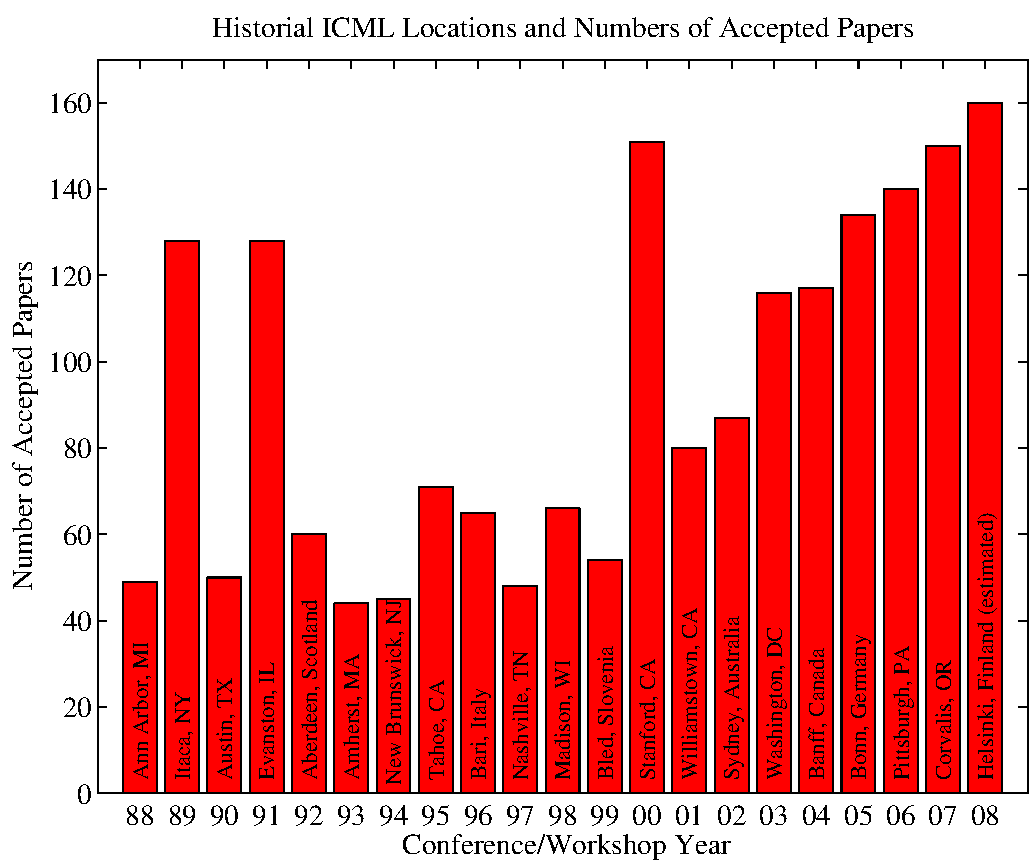
\includegraphics[width=\columnwidth]{icml_numpapers}}
\caption{Historical locations and number of accepted papers for International
  Machine Learning Conferences (ICML 1993 -- ICML 2008) and
  International Workshops on Machine Learning (ML 1988 -- ML
  1992). At the time this figure was produced, the number of
  accepted papers for ICML 2008 was unknown and instead estimated.}
\label{fig:sample-graph}
\end{center}
\vskip -5mm
\end{figure} 

\begin{table}[tb]
\vskip 3mm
\begin{center}
\begin{small}
\begin{sc}
\begin{tabular}{lcccr}
\hline
\abovespace\belowspace
Data set & Naive & Flexible & Better? \\
\hline
\abovespace
Breast    & 95.9$\pm$ 0.2& 96.7$\pm$ 0.2& $\surd$ \\
Cleveland & 83.3$\pm$ 0.6& 80.0$\pm$ 0.6& $\times$\\
Glass2    & 61.9$\pm$ 1.4& 83.8$\pm$ 0.7& $\surd$ \\
Credit    & 74.8$\pm$ 0.5& 78.3$\pm$ 0.6&         \\
Horse     & 73.3$\pm$ 0.9& 69.7$\pm$ 1.0& $\times$\\
Meta      & 67.1$\pm$ 0.6& 76.5$\pm$ 0.5& $\surd$ \\
Pima      & 75.1$\pm$ 0.6& 73.9$\pm$ 0.5&         \\
\belowspace
Vehicle   & 44.9$\pm$ 0.6& 61.5$\pm$ 0.4& $\surd$ \\
\hline
\end{tabular}
\end{sc}
\end{small}
\caption{Classification accuracies for naive Bayes and flexible 
Bayes on various data sets.}
\label{tab:sample-table}
\end{center}
\vskip -3mm
\end{table}





\section{Interim conclusions}
\label{sec:concl}
What have you learned so far?  Do the experiments indicate that the project is feasible?  Do the experiments indicate that you should consider changes to your original plan?  Can you compare your results so far to what has been reported in the literature?

\section{Plan}
\label{sec:plan}
Based on what you have done so far, present a plan for the rest of the project.  Are there any changes to the objectives?  What are the risks?  Do you need a backup plan?

\bibliography{example-refs}

\end{document} 

